\begin{figure}[htbp]\centering
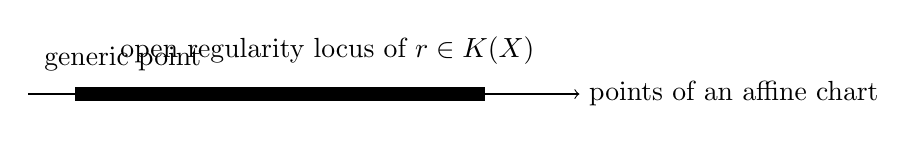
\begin{tikzpicture}
\draw[->] (0,0)--(7,0) node[right]{points of an affine chart};
\draw[line width=5pt] (0.6,0)--(5.8,0);
\fill (1.2,0) circle (2pt) node[above=5pt]{generic point};
\node at (3.8,0.55){open regularity locus of $r\in K(X)$};
\end{tikzpicture}
\caption{A rational function is regular on a dense open neighborhood of the generic point.}\label{fig:vi27-regular-locus}\end{figure}
